\section{FSW Execution Backup and Restore}\label{sec:das-exec-restore}
In \autoref{sec:bbpsim-charact}, the most important characteristics of the BBPSim environment were discussed. In particular, it was seen that the flight software was a multithreaded application running inside the \gls{BBPSim} environment. Because simulations had to run on a Linux machine, the re-implementation of the threading API by BBPSim was built on top of the POSIX threads library (\textit{pthread}), which is extensively supported by Linux. 

Saving the execution "point" of each thread was an important part of the design of the checkpointing feature in BBPSim. At restore time, it was vital to put back the threads' execution to the point they were in the code. However, playing with threads was not trivial, since they are an entity that is mostly abstracted in C code.

In this section, some approaches that attempted to resolve the execution restore problem are first of all described, along with why they didn't work or couldn't apply in the case of BBPSim. Then, a description of the checkpointing, saving and restoring operations that were adopted in this thesis is given, together with how they justify the addition of the last two necessary conditions (2 and 3) given in \autoref{sec:conditions}. 

\subsection*{Possible Solutions}
For simplicity purposes, it is often more useful to reduce the complexity of the problem and then scale up the solution to apply it in the real world. In the case of this thesis, the single-thread restore had to first be solved before attacking the multithread aspect. 

Inside a simulation, when monitoring between steps, a flight software thread in BBPSim could hold one of three possible states:
\begin{itemize}
	\item \textbf{Fresh}. This meant the thread was created (using the Deos API function \texttt{createThread()}) at the previous step but never actually given CPU time to execute. The thread is pending on a signal (a semaphore).
	\item \textbf{Mature}. The thread has executed for at least one step. This implies that it called \texttt{waitUntilNextPeriod()} at least once.
	\item \textbf{Dead}. This meant the thread was terminated at the last step, either by itself or another running thread.
\end{itemize}

Three different strategies were attempted to solve the execution restoring problem. One can take \autoref{code:example-task} on page \pageref{code:example-task} as an example of a flight task loop.
\begin{enumerate}
	\item \textbf{Restart back mature threads from scratch}. This had obvious problems.  Cold-starting all the threads alive when restoring would mean the task preamble (everything \textit{before} the infinite loop) would get executed twice: once at the first simulation and a second time when restoring. Since embedded utilities like mutexes also got restored, the flight software would try to re-create them when restoring. This would inevitably create runtime errors.
	
	\item \textbf{"Replay" the mature threads until their first \texttt{waitUntilNextPeriod()}}. This implied that the \texttt{create*()} Deos API functions had to somehow be "skipped", such that no embedded utility was created. The thread would then be replayed until its \texttt{waitUntilNextPeriod()}.
	
	Since \gls{BBPSim} was an \gls{ELF} dynamic library, this option consisted in hooking on these API calls, and redirecting them to stub functions that did nothing. The strategy was possible by using a complex set of operations that overwrote addresses in the look-up table used to resolve dynamic library function addresses, the \texttt{.rel.plt} section.\cite{online:shoumikhin}.
	
	This would have been a good solution, if only for the fact that tasks could contain more than one \texttt{waitUntilNextPeriod()}. There was nothing prohibiting a task to call \texttt{waitUntilNextPeriod()} in its preamble, for example. There was actually many occurrences of this in the flight software, for instance when threads wait for messages from other threads before starting their own task loop.
	
	With this in mind, it was necessary to find out at \textit{which} instance of \texttt{waitUntilNextPeriod()} the thread was saved, and when exactly should the Deos API be "re-enabled". This was considered as a poor approach with too many corner cases to implement effectively.
	
	\item \textbf{Reconstruct the entire threads}. This was the candidate kept for this thesis. Choosing this solution implied that everything required to reconstruct the thread needed to be included in the checkpointing artifact, hence the last two necessary conditions of \autoref{sec:conditions}. 
	
	The process relied on two facts: 1.\pathmono{libBbpSim.so} was always loaded at the same address by the dynamic linker and 2. both saved and restored simulations were ran on the same x86-64 machine. 
\end{enumerate}

In the previous sections, it was seen that, to restore back a simulation to its previous state, one had to backup two components pertaining to flight software execution: 1. one set of CPU registers per thread and 2. one execution stack per thread. In the following sections, the strategy used to gather these components is further detailed.

\subsection*{Checkpointing the CPU Register Set}
The first step in saving a thread's execution state was to come up with a way to make the flight software code checkpoint itself. In particular, it was important to obtain, at the end of every simulation step, a set of registers associated with that thread.

Saving such a register set was absolutely necessary to restore the flight threads without stability issues. The registers contained very important information about what the thread was doing. In particular, this set contained the \textit{program counter}, pictured in \autoref{fig:x86-regs}, which itself held the address of the machine instruction the thread would be currently executing. The register set also contained the stack pointer, which pointed on top of the thread's execution stack.

For obvious reasons, it was vital to save this register set \textit{at the right time} in the execution. If the registers were snapshotted at the wrong moment, the program counter would not be pointing to a viable instruction, which would make the restore operation crash. This problem was highlighted by the way thread scheduling was implemented in BBPSim.

In \autoref{fig:step-cmd}, it was shown that flight software threads were executed one after another at every simulation step. In practice, this mechanism was implemented with two semaphores. The thread was pending on a "go" semaphore inside BBPSim's \texttt{waitUntilNextPeriod()} reimplementation. Once the scheduler posted the semaphore, the thread executed a task loop until it returned inside the \texttt{waitUntilNextPeriod()} function, which signaled back to the scheduler that the thread was done. This procedure is shown in \autoref{code:thr-sched-bbpsim}.

\begin{listing}[htpb]
	\centering
	\begin{minipage}{.5\textwidth}
	\begin{minted}{c}
void Task() {
	// task premable here
	
	while(true) {
		// task loop here
		waitUntilNextPeriod();
	}
}
	\end{minted}
	\end{minipage}%
	\begin{minipage}{.5\textwidth}
	\begin{minted}{c}
//re-implementation of Deos API
void waitUntilNextPeriod() {
	//loop finished, signal returned
	sem_post(&return_sem);
	//wait for go from scheduler 
	sem_wait(&go_sem);
}
	\end{minted}
	\end{minipage}
	\caption{Thread scheduling procedure in BBPSim.}
	\label{code:thr-sched-bbpsim}
\end{listing}

If the register snapshot happened after a simulation step (using \mintinline{c}|ptrace()| like \gls{CRIU} in \autoref{sec:criu}), all the threads would be waiting inside the \mintinline{c}{sem_wait()} function, which relied on a semaphore artifact that would not be valid anymore at restore time. Therefore, another approach was needed.

The solution chosen for this problem needed the thread to checkpoint \textit{itself}, in order to gather its own set of register from within its own domain (i.e. inside DAS code). There was however another issue. Because of requirement U02, no modification to the flight software was allowed to add this snapshotting code. 

In the end, the strategy taken was the injection of checkpointing code within the flight software. By redefining the \texttt{waitUntilNextPeriod()} symbol, it was possible to inject code that would save the registers at the right moment. This could be done by using the compiler's preprocessor to convert source code before actually compiling the code, like in \autoref{code:chkpt-inject}. By harnessing the C library's types and functions for user-implemented context switching\cite{online:getcontext}, this injection would transform the flight software \ul{at compilation} to checkpoint itself at the end of every loop, before calling the real \texttt{waitUntilNextPeriod()}. 
\begin{listing}[htpb]
	\centering
	\begin{minted}{c}
#define waitUntilNextPeriod()                         \
do                                                    \
{                                                     \
	ucontext_t* chkpt = GetThreadCheckpointSaveSlot();\
	getcontext(chkpt);                                \
	waitUntilNextPeriodReal();                        \ 
} while(0)

void waitUntilNextPeriodReal()
{
	//semaphore signaling here
}
	\end{minted}
	\caption{Injection of checkpointing code in the flight software.}
	\label{code:chkpt-inject}
\end{listing}

This had big benefits, because register snapshots (done with \mintinline{c}|getcontext()|) would be done inside flight software code, and would thus enable BBPSim to restart back the execution inside the task loop, where the thread would then call \texttt{waitUntilNextPeriodReal()} to wait for the scheduler's "go" signal.

Because the \gls{BBPSim} library would always be loaded at the same address, the program counter that would get saved at this stage would still be valid at restore time. It didn't matter if this was the first simulation or a second restored simulation, the PC would remain valid in-between because it would be pointing to the same instruction. 

This effectively satisfied the second necessary condition for a stable restore, defined in \autoref{sec:conditions}, which is to save to save the register set of all threads.

\subsection*{Accessing Thread Execution Stacks}

When the program is executed, each section gets copied contiguously inside the virtual memory address range allocated for the program by the operating system. 
tried several techniques to save/restore execution stacks:
- strat 3 complicated version of longjmp: how to save execution (asm, disassembly of code, save sp, etc.% https://cs.brown.edu/courses/cs033/docs/guides/x64_cheatsheet.pdf)
Depends on the ABI

\begin{figure}[htbp]
	\centering
	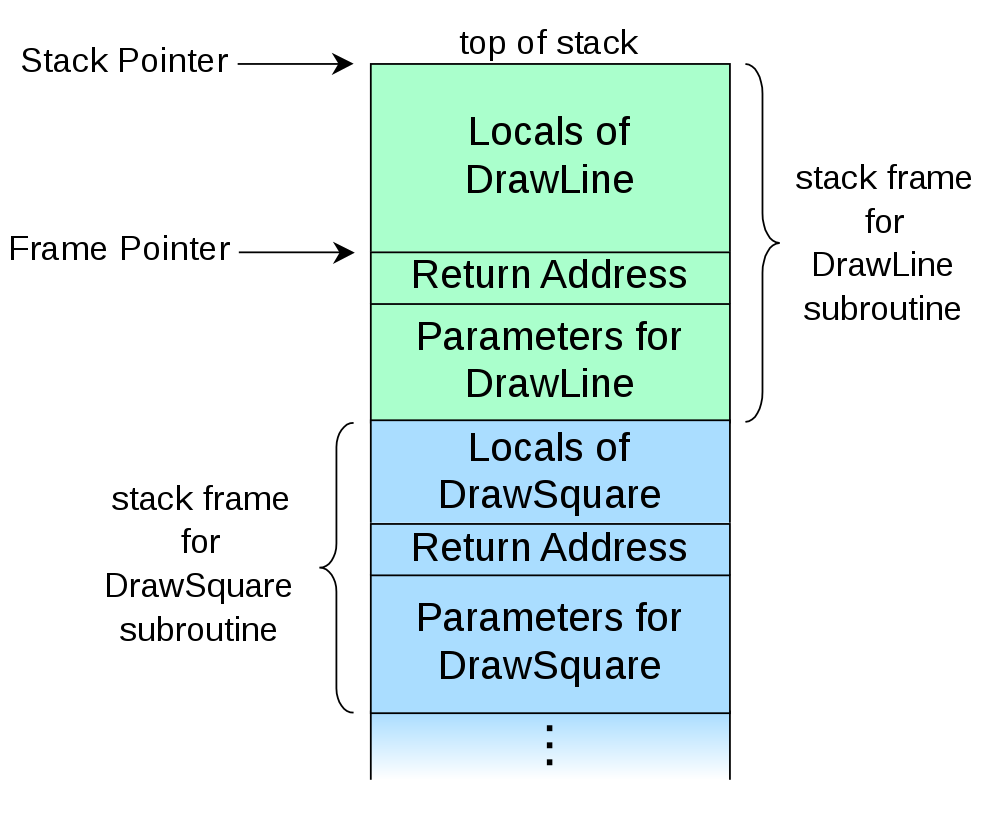
\includegraphics[width=.6\linewidth,keepaspectratio]{art/call-stack-layout.png}
	\caption{Call stack layout for upward-growing stacks\cite{online:stack-img}}
	\label{fig:call-stack-layout}
\end{figure}